%% USEFUL LINKS:
%% -------------
%%
%% - UiO LaTeX guides:          https://www.mn.uio.no/ifi/tjenester/it/hjelp/latex/
%% - Mathematics:               https://en.wikibooks.org/wiki/LaTeX/Mathematics
%% - Physics:                   https://ctan.uib.no/macros/latex/contrib/physics/physics.pdf
%% - Basics of Tikz:            https://en.wikibooks.org/wiki/LaTeX/PGF/Tikz
%% - All the colors!            https://en.wikibooks.org/wiki/LaTeX/Colors
%% - How to make tables:        https://en.wikibooks.org/wiki/LaTeX/Tables
%% - Code listing styles:       https://en.wikibooks.org/wiki/LaTeX/Source_Code_Listings
%% - \includegraphics           https://en.wikibooks.org/wiki/LaTeX/Importing_Graphics
%% - Learn more about figures:  https://en.wikibooks.org/wiki/LaTeX/Floats,_Figures_and_Captions
%% - Automagic bibliography:    https://en.wikibooks.org/wiki/LaTeX/Bibliography_Management  (this one is kinda difficult the first time)
%%
%%                              (This document is of class "revtex4-1", the REVTeX Guide explains how the class works)
%%   REVTeX Guide:              http://www.physics.csbsju.edu/370/papers/Journal_Style_Manuals/auguide4-1.pdf
%%
%% COMPILING THE .pdf FILE IN THE LINUX IN THE TERMINAL
%% ----------------------------------------------------
%%
%% [terminal]$ pdflatex report_example.tex
%%
%% Run the command twice, always.
%%
%% When using references, footnotes, etc. you should run the following chain of commands:
%%
%% [terminal]$ pdflatex report_example.tex
%% [terminal]$ bibtex report_example
%% [terminal]$ pdflatex report_example.tex
%% [terminal]$ pdflatex report_example.tex
%%
%% This series of commands can of course be gathered into a single-line command:
%% [terminal]$ pdflatex report_example.tex && bibtex report_example.aux && pdflatex report_example.tex && pdflatex report_example.tex
%%
%% ----------------------------------------------------


\documentclass[english,notitlepage,reprint,nofootinbib]{revtex4-1}  % defines the basic parameters of the document
% For preview: skriv i terminal: latexmk -pdf -pvc filnavn
% If you want a single-column, remove "reprint"

% Allows special characters (including æøå)
\usepackage[utf8]{inputenc}
% \usepackage[english]{babel}

%% Note that you may need to download some of these packages manually, it depends on your setup.
%% I recommend downloading TeXMaker, because it includes a large library of the most common packages.

\usepackage{physics,amssymb}  % mathematical symbols (physics imports amsmath)
\include{amsmath}
\usepackage{graphicx}         % include graphics such as plots
\usepackage{xcolor}           % set colors
\usepackage{hyperref}         % automagic cross-referencing
\usepackage{listings} % display code
\usepackage{subfigure}        % imports a lot of cool and useful figure commands
% \usepackage{float}
%\usepackage[section]{placeins}
\usepackage{algorithm}
\usepackage[noend]{algpseudocode}
\usepackage{booktabs}
\usepackage{subfigure}
\usepackage{tikz}
\usepackage{mathtools}
\usepackage{nccmath}
\usetikzlibrary{quantikz}
\parskip=5pt plus 1pt
\usepackage{xurl}
% defines the color of hyperref objects
% Blending two colors:  blue!80!black  =  80% blue and 20% black
\hypersetup{ % this is just my personal choice, feel free to change things
    colorlinks,
    linkcolor={red!50!black},
    citecolor={blue!50!black},
    urlcolor={blue!80!black}}

% ===========================================


\begin{document}

\title{\LARGE{Project 2: Feed Forward Neural Network}\\
  \large Classification and Regression, from linear and \\ logistic regression to neural networks}
\author{Adele Zaini}
\thanks{GitHub profile: \href{https://github.com/adelezaini/}{ https://github.com/adelezaini/}}
\date{\today}                             % self-explanatory
\noaffiliation                            % ignore this, but keep it.

\maketitle
\section{Abstract}

An implementation of a Neural Network, as Deep Learning technique, is presented. It is explored in comparison with regression methods, such as Linear and Logistic Regression, in order to appreciate the advantages of this alternative technique. Due to its architecture divided into several layers, the Neural Network can indeed lead to important improvements into the non-linear field and a good efficiency in the operations. In the present work optimizations of the related algorithm of the Stochastic Gradient Descent (SGD) and the parametrization of the network are explored. For the SGD implementation, the Ordinary Least Square (OLS) Regression shows an optimized performance for a learning rate of $10^{-5}$, $12$ minibatches and $150$ epochs, while the Ridge Regression has as optimal parameters $50$ minibatches, $150$ epochs and the two hyperparameters $\lambda = 1.87\ 10^{-4}$ and $\eta = 4.33 \ 10^{-4}$. In the Regression case, the Neural Network best performs with $\eta=0.001$ and $\lambda \in [10^{-12},0.001]$, while in the Classification case it has a good flexibility on the parameters choice, but the accuracy score never exceeds the threshold of $41\%$. While the choice of the activation function does not influence much the performance of the network, the architecture setting can lead to interesting variations. The optimal performance is found choosing few hidden layers with the number of neurons that starts close to the input size and approaches progressively the output size. 

% ===========================================
\section{Introduction}
The neural network, also known as artificial neural network, is a subset of machine learning techniques and is at the heart of Deep Learning algorithms. Its name and structure is inspired by the human brain, mimicking the way that biological neurons interact to one another. The very powerful point of this technique is that it can explore new ways of analysing and interpreting data, that are limited by the classical methods, such as regression ones. 

In this report, we will implement a Feed Forward Neural Network with backpropagation and Stochastic Gradient Descent (SGD) in Python. We will firstly concentrate on a preliminary step for the implementation that is the optimization technique of SGD. Afterwards the focus is on the implementation of the Neural Network class both in the Regression and Classification cases, while exploring the optimization of different hyperparameters and network architectures. Comparisons with Linear and Logistic Regression will be performed to check the results.

The report is organized as follows. After this introduction, the methods are explored considering the background theory and the algorithms implemented. The following section will present the results of the work, while commenting and discussing them. The final section is to summarize the analysis into the conclusions and to have an overview on future perspective.


    
% ===========================================

\section{Methods} \label{sec:methods}
\subsection{Theory and algorithms} \label{sec:theory}

The basic idea of Neural Network lies on building a system of interconnected units, called \textit{neurons}, divided in multiple layers, that broadcast signals throughout the neural system. The structure is composed of an input layer, one or more hidden layers, with different number of neurons in each of them, and the output layer. The broadcasting of the signal happens thanks to \textit{activation functions} that elaborate the input signals for each neuron into the ouput ones. They are coupled with weights and biases associated to each neuron so that the output is more or less relevant when broadcasted to the next layer. This process starts from the input layer and it runs thoughtout each neuron of each layer, until resulting into an output layer, that is the model prediction (i.e.\textit{Feed Forward Neural Network}). The next step is to \textit{train} the network. Given already the expected \textit{true} output, it is compared to the model prediction thanks to a \textit{cost function} that evaluates the performance of the model. The aim is to minimize this value and using the \textit{backpropagation} and Stochastic Gradient Descent algorithms, is possibile to optimize the parameters (i.e. weights and biases) to have the closest result to the expected one. This last step is extremely important because then the network is able to \textit{predict} the results given any other input data. The overall performance of the network is evaluated thanks to the \textit{metrics} on a test dataset.

\begin{figure}[h]
    \centering 
    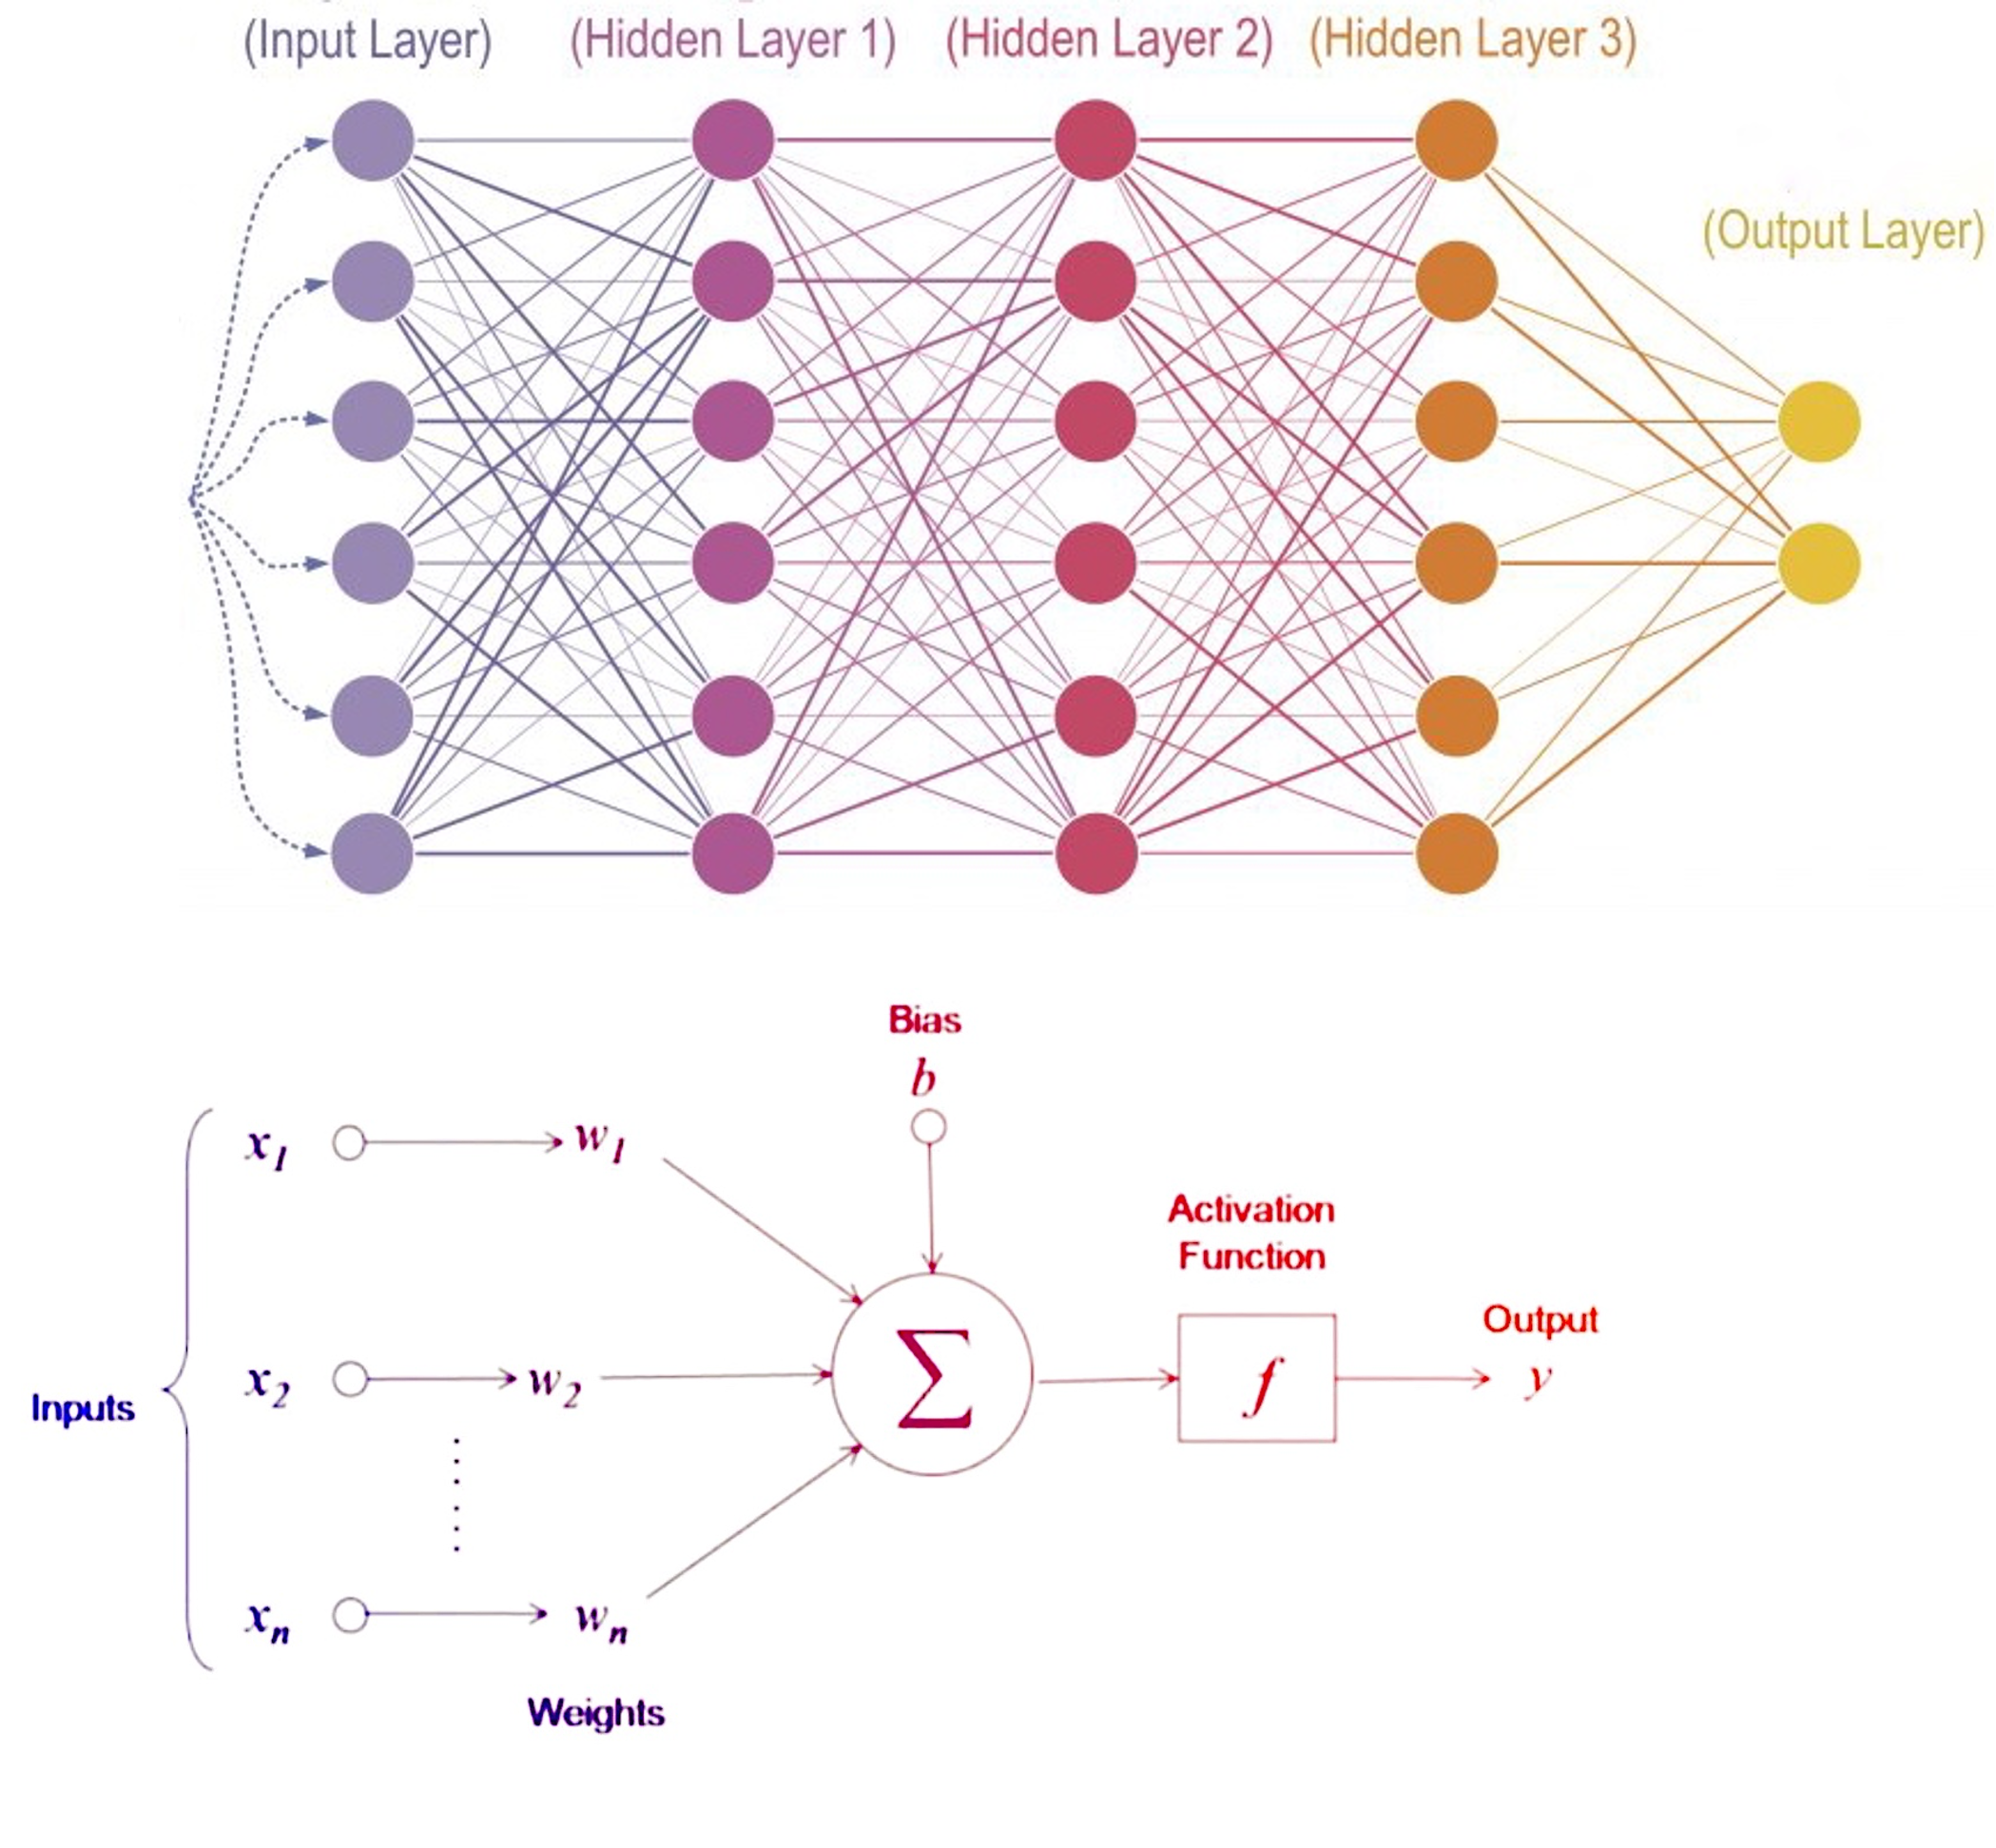
\includegraphics[scale=0.5]{neural_network_structure.png}
    \caption{Examples of Neural Network architecture, with several neurons divided into the hidden layers and with a focus on one single neuron and its schematic operation.}
    \label{fig:nn}
\end{figure}
\textbf{Feed Forward Neural Network} – 
The key idea of this type of Neural Network is that the information moves in only one direction: forward through the layers. As depicted in Figure \ref{fig:nn}, each single neuron has $\{x_i\}$ as input data, which is linearly combined  with the respective weights $\{w_i\}$ and biases $\{b_i\}$ (it can be a single value for all the neurons of the layer or different values): $z=\sum_i (w_i x_i + b_i)$ .

The output $y$ is produced via the activation function $f$ as follows:
\begin{equation}
y = f\left(\sum_{i=1}^n w_ix_i + b_i\right) = f(z),
\end{equation}

In a dense FFNN with multiple neurons and hidden layers, the inputs $\{x_i\}$ are the outputs of
the neurons in the preceding layer, and the output $y$ is one of the inputs for the next layer. At the end, the equation results to be:

%\begin{equation}
\begin{multline}
    y^{L+1}_i = f^{L+1}\left[\!\sum_{j=1}^{N_L} w_{ij}^3 f^L\left(\sum_{k=1}^{N_{L-1}}w_{jk}^{L-1}\left(\dots \\ f^1\left(\sum_{n=1}^{N_0} w_{mn}^1 x_n+ b_m^1\right)\dots\right)+b_k^2\right)+b_1^3\right] 
    \label{completeNN} \tag{14}
\end{multline}
%\end{equation}

where $L$ is the number of hidden layers.

\textbf{Back propagation} – 
The back propagation is the core algorithm behind how neural networks learn. After a first forward run thoughout the network, to have the first attempt of a prediction, the network needs to be trained. In other words, it means that the parameters (i.e. weights and biases) need to be optimized to minimize the cost function, which quantifies the difference between the model output and the expected output values.

The idea behind this algorithm is to go back thoughout the network, layer by layer, using the \textit{chain rule} to find the optimal parameters. This algorithm can be coupled with different optimization techniques that evaluate the partial derivatives for the chain rule.

The starting point is at the end of the network: evaluating the total error $\hat{\delta}^L$ of the output layer by computing all $\delta_j^L$ for each outputs:
$$
\delta_j^L = f'(z_j^L)\frac{\partial {\cal C}}{\partial (a_j^L)}.
$$

Then the back propagate error is computed for each $l=L-1,L-2,\dots,2$ layer as

$$
\delta_j^l = \sum_k \delta_k^{l+1}w_{kj}^{l+1}f'(z_j^l).
$$

Finally, the weights and the biases are updated using an optimization tecnique for each $l=L-1,L-2,\dots,2$, such as the \textit{Gradient Descent} algorithm or one of its variant:
$$
w_{jk}^l\leftarrow  = w_{jk}^l- \eta \delta_j^la_k^{l-1},
$$
$$
b_j^l \leftarrow b_j^l-\eta \frac{\partial {\cal C}}{\partial b_j^l}=b_j^l-\eta \delta_j^l,
$$
where $\eta$ is the learning rate.

The backpropagation is an algorithm for determining how a single training example would like to nudge the weights and biases, in terms of what relative proportions to those changes cause the most rapid decrease to the cost function. But this algorithm needs to be run over all the examples (i.e. datapoints for the Regression case and digits/images for the Classification case), this is why it is convenient to use \textit{Stochastic Gradient Descent} with mini-batches with an outer loop that steps through multiple epochs of training (see below).

\textbf{Activation functions} – 
The choice of the activation functions is a key element in the performance of the network. The classical choice is the \textit{sigmoid} function:
$$
f(x) = \frac{1}{1 + e^{-x}},
$$
but in the past it has been shown its limits for large input values (i.e. \textit{vanishing gradient problem} in applying the back propagation algorithm). Other choices can be: \textit{hyperbolic tangent}, \textit{ReLU (Rectified exponential Linear Unit)}, \textit{eLU (exponential Linear Unit)}, \textit{Leaky ReLU}...

For the output layer the most common activation function is the \textit{softmax}:
$$
f(z_i) = \frac{e^{z_i}}{\sum_{j=1}^K e^{z_j}}.
$$
While in the Regression case, no activation function is needed for the output layer.

\textbf{Cost function and metrics}  – 
The \textbf{cost function} (or loss function) is a method of evaluating how well the neural network fits the dataset or, in other words, it quantifies the error between the predicted output values and the expected ones. It is used to in the training process to optimize the paramaters in order the get to the minimum of this function. Depending on the problem, the cost function can have different expressions. The most common choice for the regression and the classification case are the Mean Squared Error (MSE) and the Cross-Entropy loss (CE) respectively.

$$
MSE(y,\hat{y}) = \frac{1}{n}
\sum_{i=0}^{n-1}(y_i-\hat{y}_i)^2,
$$
where $\hat{y}_i$ is the predicted value of the $i-th$ sample, $y_i$ is the corresponding true value and $n$ is the total number of datapoints.

$$
CE = -
\sum_{c=1}^{M}(y_c \ \mathsym{log}(p_c)
$$

where $y_c$ is the binary indicator (0 or 1) if the class label $c$ is the correct classification label, $p_c=$ is the predict probability of the class $c$ (i.e. output value before filtered by the output activation function).

The \textbf{metrics} is a function that evaluates the overall performance of the neural network. It's a similar concept to the cost function, but while the cost function is used on the training dataset to optmize the neural network parameters (i.e. it quantifies the \textit{in-sample error}), the metrics is used on test datasets at the end of the training process (i.e. it quantifies the \textit{out-of-sample error}). There are different expressions for the metrics too. For the regression and the classification cases, the MSE and the Accurancy score are the most in use.
$$
\text{Accuracy} = \frac{\sum_{i=1}^n I(t_i = y_i)}{n} ,
$$

Here $t_i$ represents the target, $y_i$ the outputs of the FFNN code, $n$ is the number of targets $t_i$ and $I$ is the indicator function: $1$ if $t_i = y_i$ and $0$
otherwise.

\textbf{Gradient Descent and Stochastic Gradient Descent} – 
The Gradient Descent (GD) is an optimization technique and the most common way to train neural networks. It is an algorithm to minimize an objective function (i.e. cost function $C(\mathbf{\beta})$) parameterized by model's parameters $\beta$ by updating the parameters in the opposite direction of the gradient of the objective function $\gradient_{\beta} C(\mathbf{\beta})$ to the parameters. It is based on the \textit{Newton-Raphson's method}, an approximation to the first order of the Taylor expansion, where the learning rate $\eta$ (i.e. inverse of the second derivative) determines the size of the steps we take to reach a (local) minimum. It is possible to demonstrate that in the matrix notation the optimal value of the learning rate is $\hat{\eta}=1 / \lambda_{max}$, where $\lambda_{max}$ is the maximum eigenvalue of the Hessian matrix, so that it grants convergence and efficiency in the iterations. In other words, iterating this "parameters update", we follow the direction of the slope of the surface created by the objective function downhill until we reach a valley (Figure \ref{fig:sgd}).
\begin{figure}[h]
    \centering 
    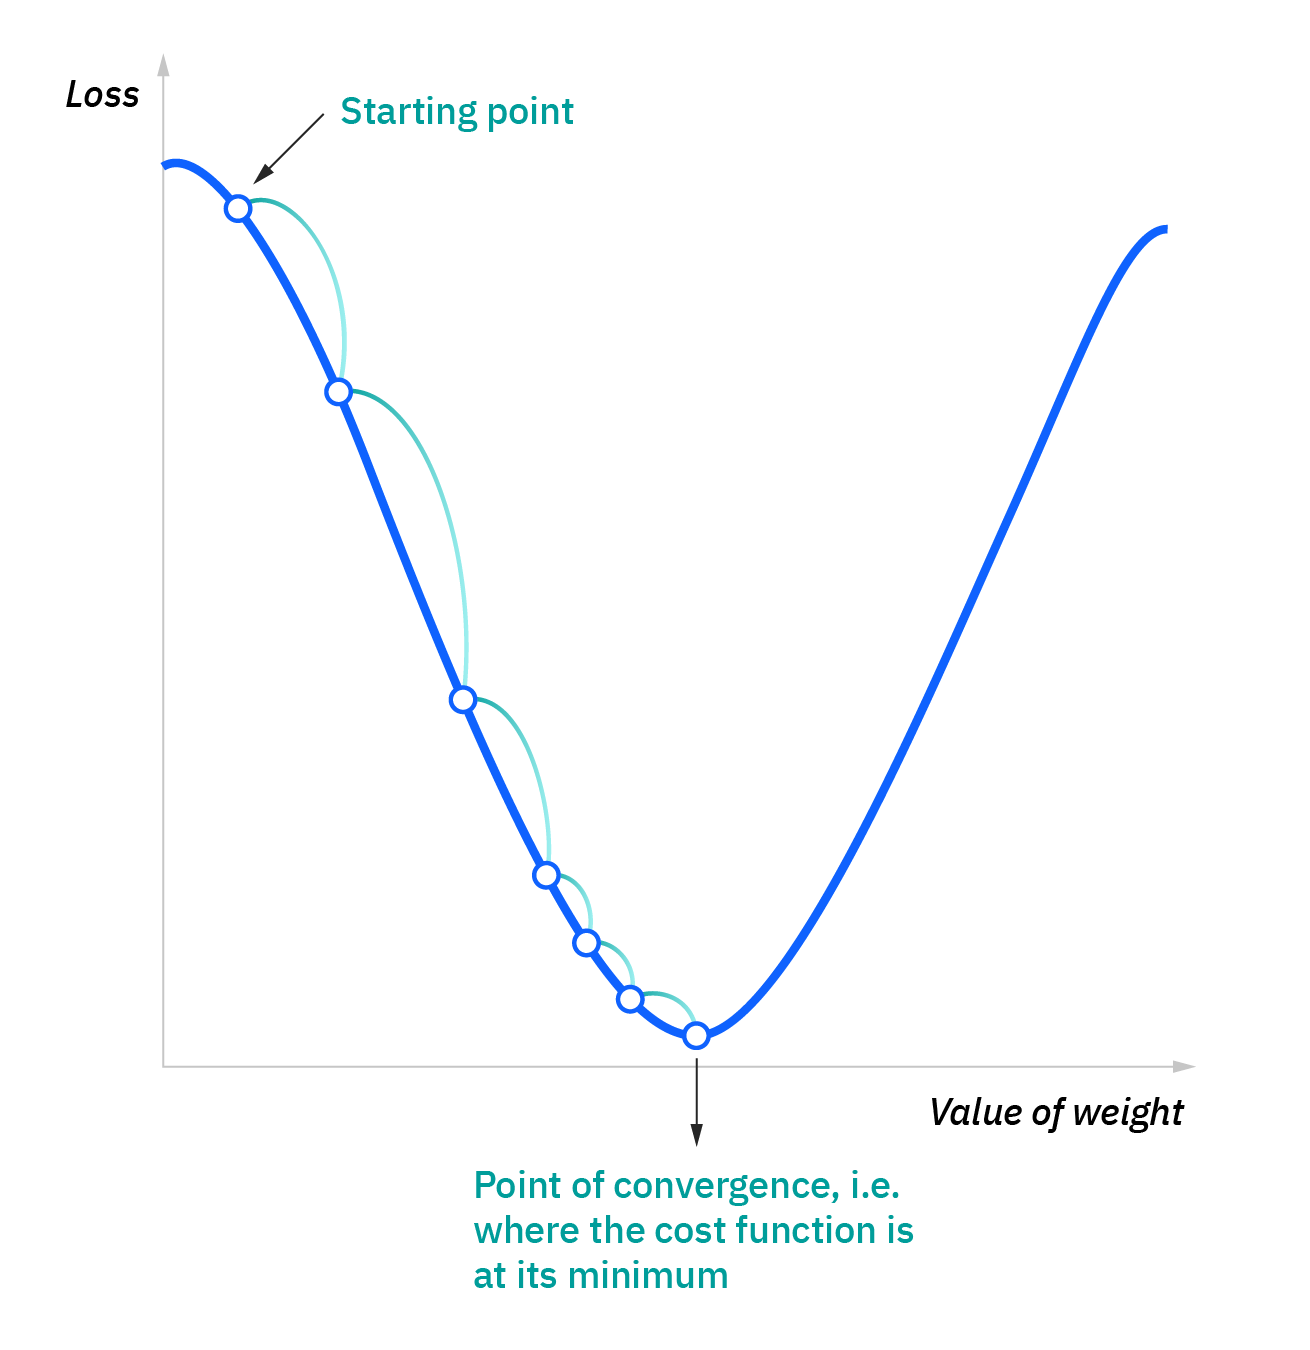
\includegraphics[scale=0.2]{SGD.png}
    \caption{Intuitive idea of the Gradient Descent optimization when updating the parameters.}
    \label{fig:sgd}
\end{figure}
Nevertheless, the Gradient Descent algorithm represents limitations connected to its characteristic of being very precise. These concerns its low efficiency and its high dependence on initial conditions that leads to be trapped in local minima. In order to improve this algorithm, "randomness" needs to be included and the way is to implement the Stochastic Gradient Descent (SGD). While in the GD the gradient is evaluated from the entire dataset, in the SGD it is calculated from a randomly selected subset of the data, called \textit{mini-batch} (Figure \ref{fig:gd_sgd}). The \textit{mini-batches} are embedded in an iteration loop over the number of \textit{epochs}.

\begin{figure}[h]
    \centering 
    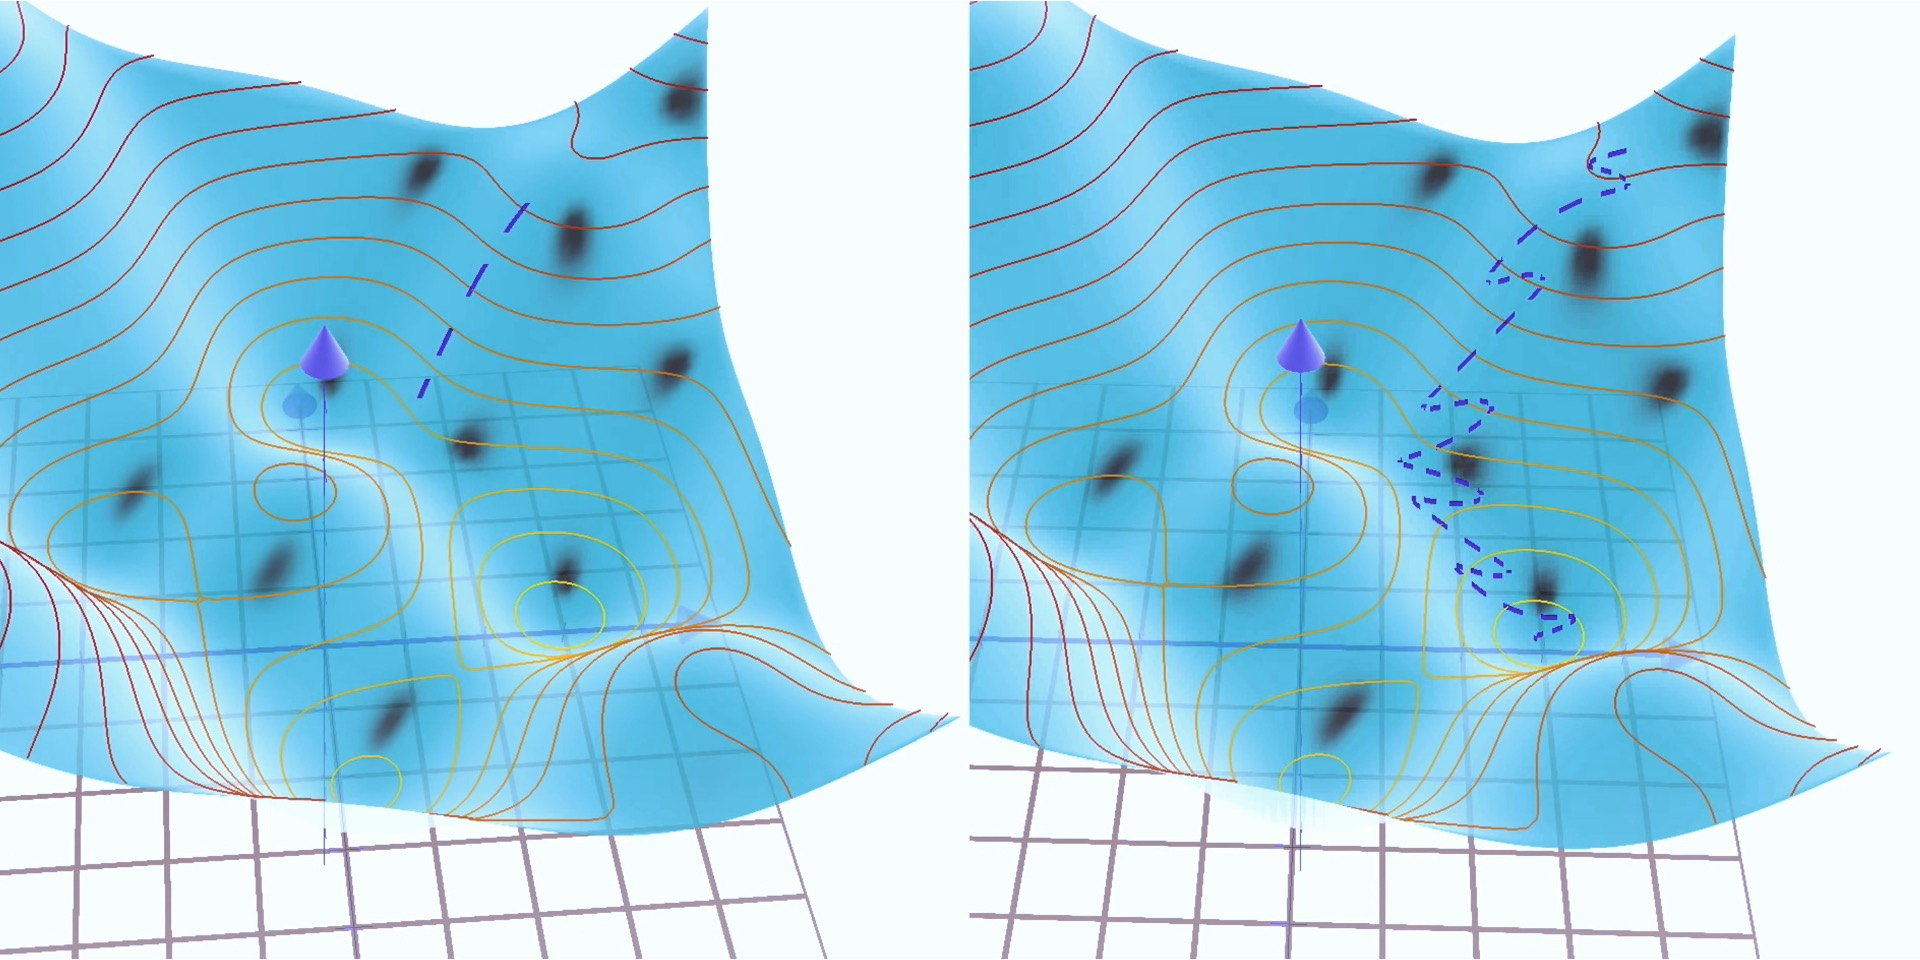
\includegraphics[scale=0.1]{GD_SGD.jpg}
    \caption{Difference of optimization paths over a two-dimensional surface: a) precise and inefficient Gradient Descent (left) and b) random and efficiency Stochastic Gradient Descent (right).}
    \label{fig:gd_sgd}
\end{figure}

\textbf{Optimizers} – There are variants of the optimization algorithms, such as SGD with momentum, AdaGrad, RMSprop, ADAM.

1. \textit{Gradient Descent}:
$$
\beta \leftarrow \beta -\eta \ \gradient C(\beta)
$$

2. \textit{Gradient Descent with momentum}:
$$
\begin{array}{c}
v \leftarrow \gamma v + \eta \ \gradient C(\beta) \\
\beta \leftarrow \beta - v
\end{array}
$$
where $\gamma$ is the \textit{drag} parameter, commonly set to $\gamma = 0.9$.

3. \textit{AdaGrad}:
$$
\begin{array}{c}
r \leftarrow r + g \odot g \\
\beta \leftarrow \beta -\frac{\eta}{\sqrt{r+\delta}} \odot g
\end{array}
$$
where $g=\gradient C(\beta)$, $\odot$ is the \textit{Hadamard product} or element-wise product and $\delta\sim10^{-8}$ is a parameter to avoid division by $0$.

4. \textit{RMSprop}:
$$
\begin{array}{c}
r \leftarrow \rho r + (1-\rho) g \odot g \\
\beta \leftarrow \beta -\frac{\eta}{\sqrt{r+\delta}} \odot g
\end{array}
$$
where $\rho$ is usually set to $0.9$.

5. \textit{ADAM}:
$$
\begin{array}{c}
\hat{m} \leftarrow [\beta_1 m + (1-\beta_1) g] / (1-\beta_1) \\
\hat{v} \leftarrow [\beta_2 v + (1- \beta_2) g^2] / (1-\beta_2) \\
\beta \leftarrow \beta -\frac{\eta}{\sqrt{\hat{v}+\delta}} \odot \hat{m}
\end{array}
$$
where $\beta_1 \sim 0.9$ and $\beta_2 \sim 0.999
$.

Moreover, the \textbf{learning rate} can be chosen as \textit{constant} value, but it can also have different \textit{learning schedules} that make the learning rate decrease during the iteration process. In this work two \textit{learning schedules} have been implemented:
\begin{enumerate}
    \item $\eta(t) = t_0 / (t+t_1)$
    \item $\eta(t) = \eta_0 / t^{p_t}$, where $p_t \sim 0.25$
\end{enumerate}
where $t$ is the iteration counter.
% ===========================================
\subsection{Code implementation}\label{sec:code}
The algorithms previously explained have been implemented in a class called \texttt{NeuralNetwork}. When initializing the class, the architecture (i.e. list of neurons and activation functions for each hidden layer) and parameters (e.g. learning rate, optimizer...) are set. The default architecture sees one hidden layer with two neurons and the  \textit{sigmoid} as activation function. If the number of hidden layers (i.e. lenght of the list of neurons) is higher than one and the activation list is composed by a single element, the class automatically set that function as the activation for each hidden layer, otherwise different activation functions can be set for different hidden layers. The activation function of the output layer is set to \texttt{None} in the regression case and \texttt{softmax} in the classification case. Exceptions are thrown if the input arguments do not meet the requirements (e.g. the activation function is not in the list of the implemented ones).

The core of the class is the \texttt{fit()} method, which receives \texttt{X} and \texttt{Y} as arguments, initializes the weights and the biases with the normal distribution $\mathsym{N}(0,n)$ (where $n$ is the number of inputs to the neuron, number of neurons of the previous layer) and trains the network. It returns the network trained and ready to predict outputs from any input dataset (\texttt{predict()} method).

The following picture shows the class structure and sequential and embedded operations in a schematic way:
\begin{figure}[h]
    \centering 
    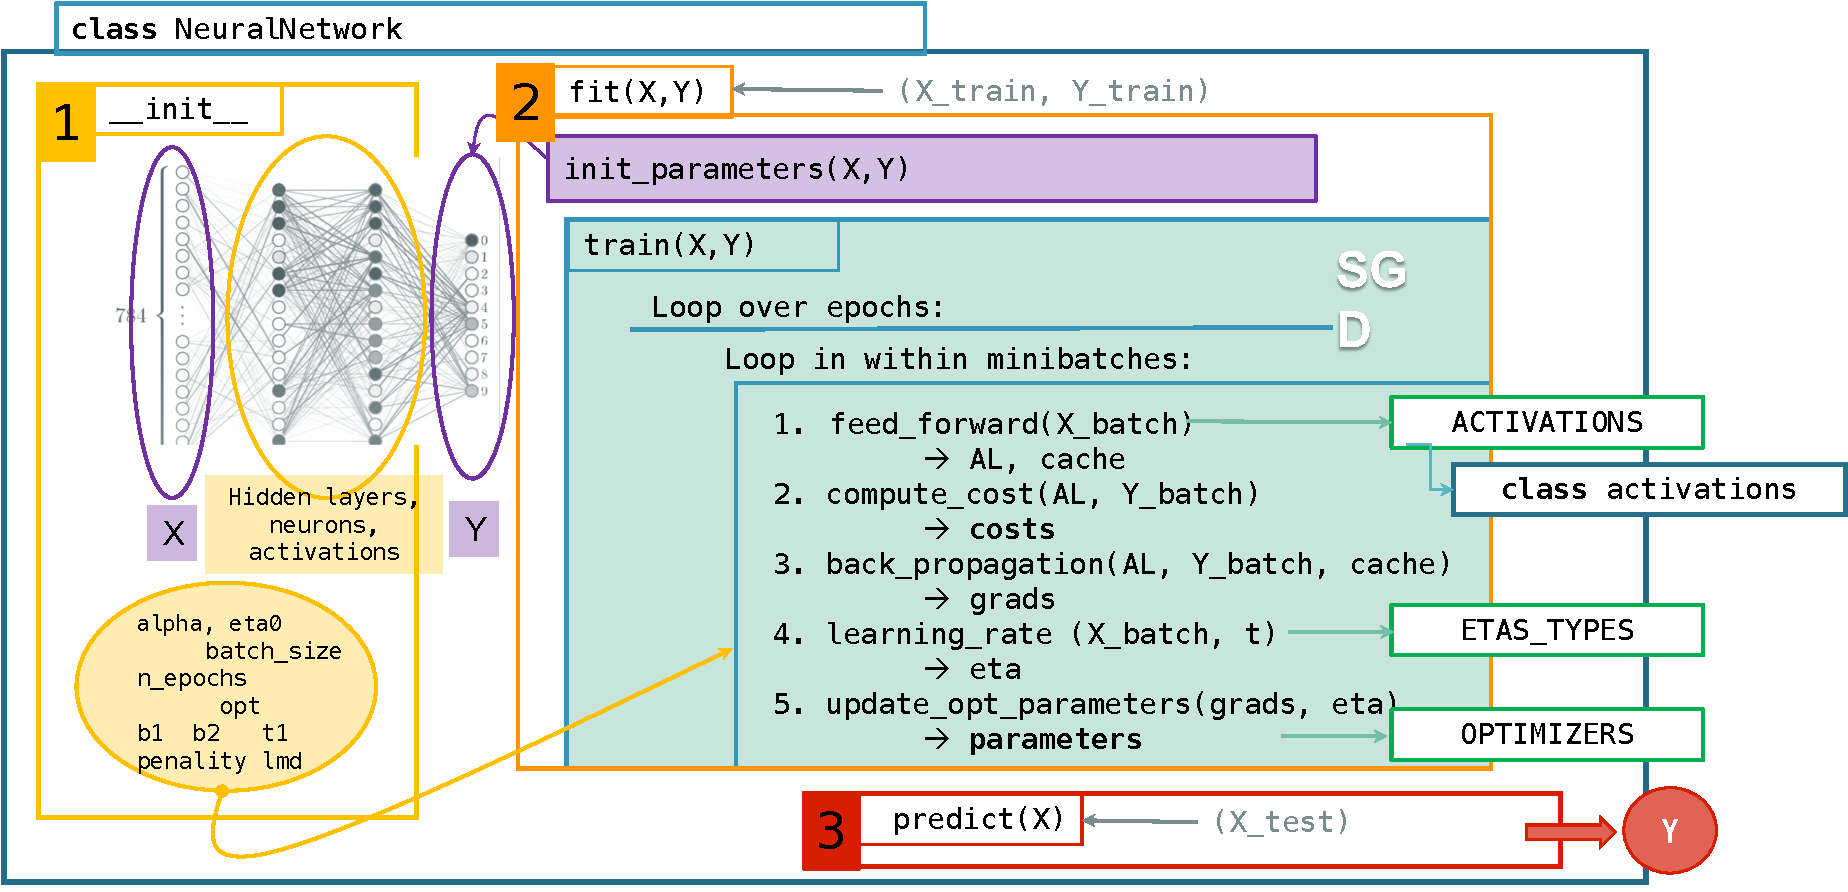
\includegraphics[scale=0.23]{FFNN.pdf}
    \caption{\texttt{\textbf{class} NeuralNetwork}: structure and methods.}
    \label{fig:ffnn}
\end{figure}

The duties of the methods are:
\begin{itemize}
    \item[–] \texttt{\_\_init\_\_()}: initialize the NN in terms of architecture (layers, neurons, activations functions) of the network and all the parameters needed for the backpropagation and the optimization algorithms.
    \item[–] \texttt{fit()}: fit the network with the given input X and output Y and initialize layers, parameters and train the network.
    \item[–] \texttt{init\_parameters()}: initialize the weights and the biases in the given architecture (i.e. [2,4,3,2] as list of number of neurons), using a normal distribution.
    \item[–] \texttt{feed\_forward()}: implements the Feed Forward algorithm
    \item[–] \texttt{compute\_cost()}: implement the cost function with optional regulation techniques 'l1' and 'l2'
    \item[–] \texttt{cost\_function()}: return the cost function specific to Regression or Classification case.
    \item[–] \texttt{backpropagation()}: implement the backward propagation
    \item[–] \texttt{learning\_rate()}: update the learning rate when it is different than a given constant value. Different types of learning rate can be chosen.
    \item[–] \texttt{update\_opt\_parameters()}: update parameters using gradient descent algorithm with the given optimizer.
    \item[-] \texttt{train()}: the core algorithm of the NN object: 1) Feed Forward to arrive to the output layer; 2) Backpropagation to evaluate all the gradients for each example/feature; 3) Update parameters (weights and biases) according to the optimizer (throughout the examples/features); 4) All wrapped up in the stochastic part (i.e. epochs and mini batches) of the SGD algorithm.
    \item[-] \texttt{predict()}: predicting values with the Feed Forward algorithm, to be used after training. The output depends on the Regression or Classification case.
    \item[-] \texttt{model\_performance():} implements the metrics specific for the Regression or Classification case.
\end{itemize}

This is the parent class of \texttt{\textbf{class NN\_Regression}} and \texttt{\textbf{class NN\_Classifier}}, which inherit all the methods, but the output activation function initialization, the cost function and the metrics implementations.

This class is coupled to another class: \texttt{\textbf{class} activations}. This is an abstract parent class, that defines two methods: \texttt{eval(X)} and \texttt{gradient(X)}. These methods are then implemented in each derivative class to evaluate the function result and the function gradient at a given \texttt{X} respectively.
The following activations functions are implemented:
\texttt{sigmoid}, \texttt{tanh}, \texttt{elu}, \texttt{relu}, \texttt{leaky\_relu}, \texttt{softmax}. In order to use this class into the \textttt{NeuralNetwork} one, a dictionary was created to collect the derivative classes and the usage is the following:

\begin{verbatim}
# Dictionary:
ACTIVATIONS = {'sigmoid': sigmoid, 'tanh': tanh,
    'relu': relu, 'leaky_relu': leaky_relu, 
    'elu': elu, 'softmax': softmax, None: None}
    
# Choose the activation functions in the NN layers:
activations_list = ['sigmoid','relu']
    ...
# In the Feed Forward loop over hidden layers (l):
act_func = ACTIVATIONS[activations_list[l]] 
Al = act_func(Zl, alpha).eval()

# When updating the paramters with the 
optimization technique:
act_func = ACTIVATIONS[activations_list[l]] 
Al = act_func(Zl, alpha).gradient()
\end{verbatim}

For any further information, the GitHub repository (\href{https://github.com/adelezaini/MachineLearning/Projects/Project2}{https://github.com/adelezaini/MachineLearning}) contains all the source code with a detailed documentation.

\textbf{Neural Network Routine} After describing the class itself, we will focus briefly on the steps needed when using neural networks to solve supervised learning problems. The routine is the following:

\begin{enumerate}
    \item \textit{Collect and pre-process data}: elaborate on the given input and output datasets in order to make them suitable for the Neural Network operations;
    \item \textit{Define model architecture, choose cost function and optimizer}: initialize the Neural Network overall structure.
    \item \textit{Initialize the model parameters}: weights and biases are initialized with a normal distribution;
    \item \textit{Train the model with the training dataset}: in a loop of a certain number of epochs and mini-batches:
    \begin{itemize}
        \item[–] Calculate current loss (forward propagation)
        \item[–] Calculate current gradient (backpropagation)
        \item[–] Update paramaters (gradient descent or another optimization algorithm)
    \end{itemize}
    \item \textit{Make prediction with the test data}: after the paramters are optimized;
    \item \textit{Evaluate model performance and adjust hyperparameters}: analysis over the several paramters in order to find the minimum of the metrics of the model.
\end{enumerate}

\textbf{Linear Regression class}
In order to solve the first task and perform comparison with the Neural Network code, a class called \texttt{LinearRegression}, and the derivative \texttt{\textbf{class} OLSRegression, RidgeRegression} and \texttt{LassoRegression}, has been implemented from the code of project 1. Methods to evaluate the optimal $\beta$ has been implemented for both the matrix-invertion evaluation and the Stocastic Gradient Descent algorithm, with the different optimizers previous exposed.
Here is the list of the methods and their duties:
\begin{itemize}
    \item[–] \texttt{\_\_init\_\_()}: create the object given the $X$ and $y$.
    \item[–] \texttt{split()}: split the data into training and test subsets.
    \item[–] \texttt{rescale()}: rescale the data using the \texttt{StardardScaler} of Scikit-Learn.
    \item[–] \texttt{solver()}: regression equation, to be implemented in each derivative class.
    \item[–] \texttt{gradient()}: gradient of the \texttt{solver}, to be implemented in each derivative class.
    \item[–] \texttt{fit()}: fit the model and return beta-values, according to the \texttt{solver}.
    \item[–] \texttt{fit\_SK()}: fit the model and return beta-values, using Scikit-Learn.
    \item[–] \texttt{fitGD()}: fit the model and return beta-values, using the Gradient Descent and calling the \texttt{gradient} method.
    \item[–] \texttt{fitSGD()}: fit the model and return beta-values, using the Stochastic Gradient Descent and calling the \texttt{gradient} method.
    \item[–] \texttt{predictSGD\_BS()}: fit the model and return beta-values, using the Stochastic Gradient Descent and the bootstrap algorithm.
    \item[–] \texttt{predict()}: predict $y$ values given an external $X$. The methods of \texttt{predict\_train()} and \texttt{predict\_test()} are analogous but they work on the internal members.
    \item[–] \texttt{rescaled\_predict}: rescale $y$ prediction to the original data range.
    \item[–] \texttt{MSE\_train()}, \texttt{MSE\_test()}, \texttt{R2\_train()}, \texttt{R2\_test()}: evaluate the MSE or the R2 score on internal members.
    \item[–] \texttt{Confidence\_Interval()}: return the confidence interval of the beta-values.
\end{itemize}
A simple example of usage is:
\begin{verbatim}
model = OLSRegression(X,y)
beta = model.split().rescale().fit()
mse = model.MSE_test()
\end{verbatim}

\textbf{Logistic Regression class}
In order to solve the last task, a draft class has been implemented for solving a Logistic Regression case to compare with the Neural Network performance. The methods are the following:
%that have been sketched
\begin{itemize}
    \item[–] \texttt{\_\_init\_\_()}: initialize the class with given $X$ and $y$.
    \item[–] \texttt{split()}: split in train and test datasets
    \item[–] \texttt{loss(()}: evaluate the cross entropy
    \item[–] \texttt{gradients()}: evaluate the gradients for the Stochastic Gradient Descent
    \item[–] \texttt{train()}: implement the Stochastic Gradient Descent
    \item[–] \texttt{predict()}: predict new output with the trained/fitted class
    \item[–] \texttt{accuracy()}: evaluate the accuracy score.
\end{itemize}

%This class hasn't tested yet because of problems that will be explained later in the report.

All the source code can be found in the GitHub repository: \href{https://github.com/adelezaini/MachineLearning/Projects/Project2}{ https://github.com/adelezaini/MachineLearning} in the directory \texttt{Projects/Project2}.


% ===========================================
\section{Results and discussion}\label{sec:results}

The work for this project is divided in different tasks. Task \textit{a} focuses on the Stochastic Gradient Descent performance, while task \textit{b, c, d} focus on exploring neural networks. Task \textit{e} regards the implementation of the Logistic Regression code.

The datasets are the {Franke Function} and the \textit{Boston Housing} for the regression case, and the \textit{Wisconsin Breast Cancer} and the \textit{MNIST digits} for the classification case.

\subsection{Stochastic Gradient Descent}

\textit{Perform an analysis of the results for OLS and Ridge regression as
function of the chosen learning rates, the number of mini-batches and
epochs as well as algorithm for scaling the learning rate.}

The dataset is generated by the Franke Function taken $n=25$ for each dimensions $(x,y)$ (total datapoints: $N=25^2=625$) with an added stochastic noise normally distributed $\mathsym{N}(0,0.1)$. The design matrix $X$ of a polynomial of \texttt{degree=5}, together with $z$, is the input to initialize the \texttt{OLSRegression} and \texttt{RidgeRegression} objects. Splitting into train and test datasets and rescaling with \texttt{StardardScaler(with\_std=False)} from Sklearn have been performed before fitting the model with \texttt{n\_epochs = 50, n\_minibatches = 10} and default hyperparameters $\lambda = 10^{-12}$ and $\eta_0 = 1 / \lambda_{max}$ ($\lambda_{max}$ is the maximum eigenvalue of the Hessian matrix of $X$). This first choice is reflected is quite poor $MSE$, that is equal to $2.18$ for both OLS and Ridge Regression, in the face of $MSE_{sk} = 0.0267$ given by the Sklearn model. These result is surely improvable with the optimization of the parameters.

The performance analysis starts with the optimization of the learning rate, evaluated with a \textit{learning schedule} dependent on two parameters $t_0$ and $t_1$. Afterwards the numbers of minibatches and epochs are explored. At the end a grid-search of learning rate and $\lambda$ gives the best combination of the Ridge case. In each step the optimal parameter found in the previous step is taken as input parameter for the next fitting.

\begin{figure}[h]
    \centering 
    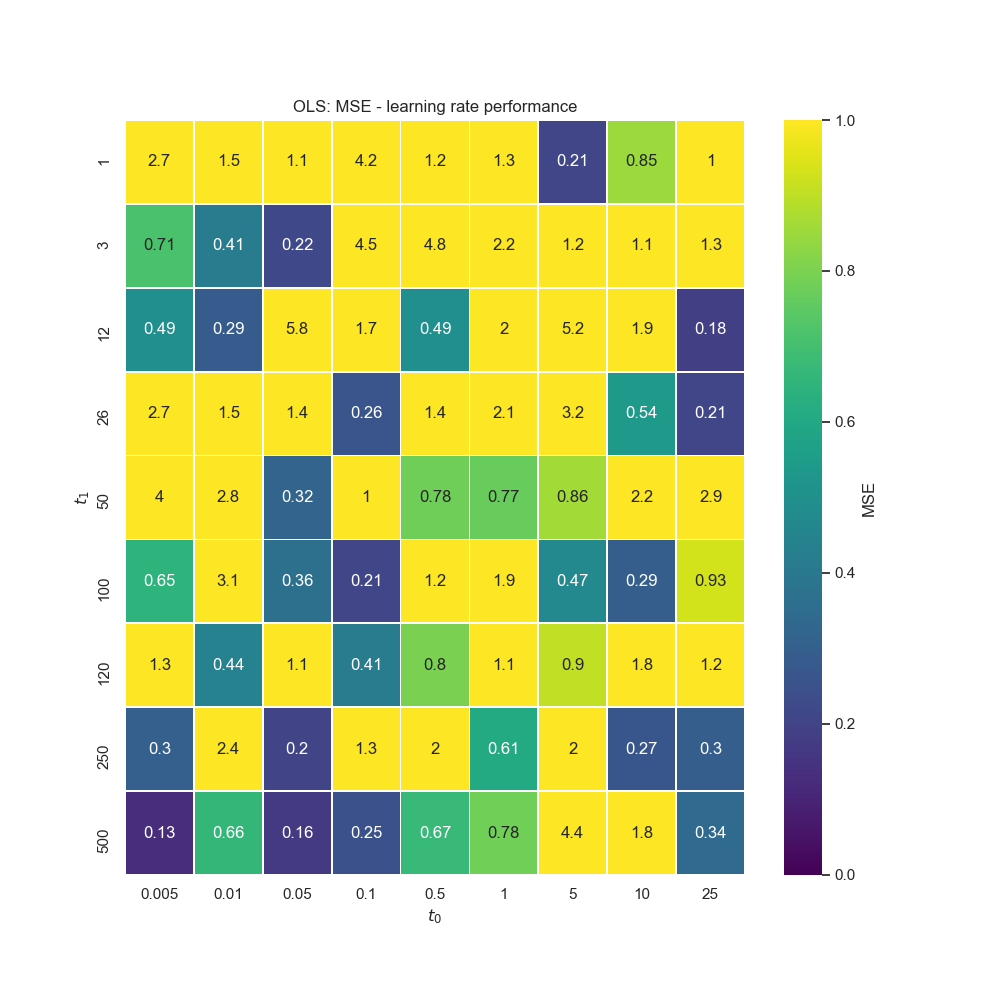
\includegraphics[scale=0.3]{SGD/SGD_eta_OLS.png}
    \caption{\textbf{Task $a$ – SGD}: MSE performance of the learning rate, choosing a \textit{learning schedule} with parameters $t_0$ and $t_1$. Maximum MSE value set to 1. The optimal values are $t_0 = 5 \ 10^{-3}$ and $t_1 = 500$, given an initial learning rate of $\eta_0=10^{-5}$.}
    \label{fig:eta0_ols}
    \centering 
    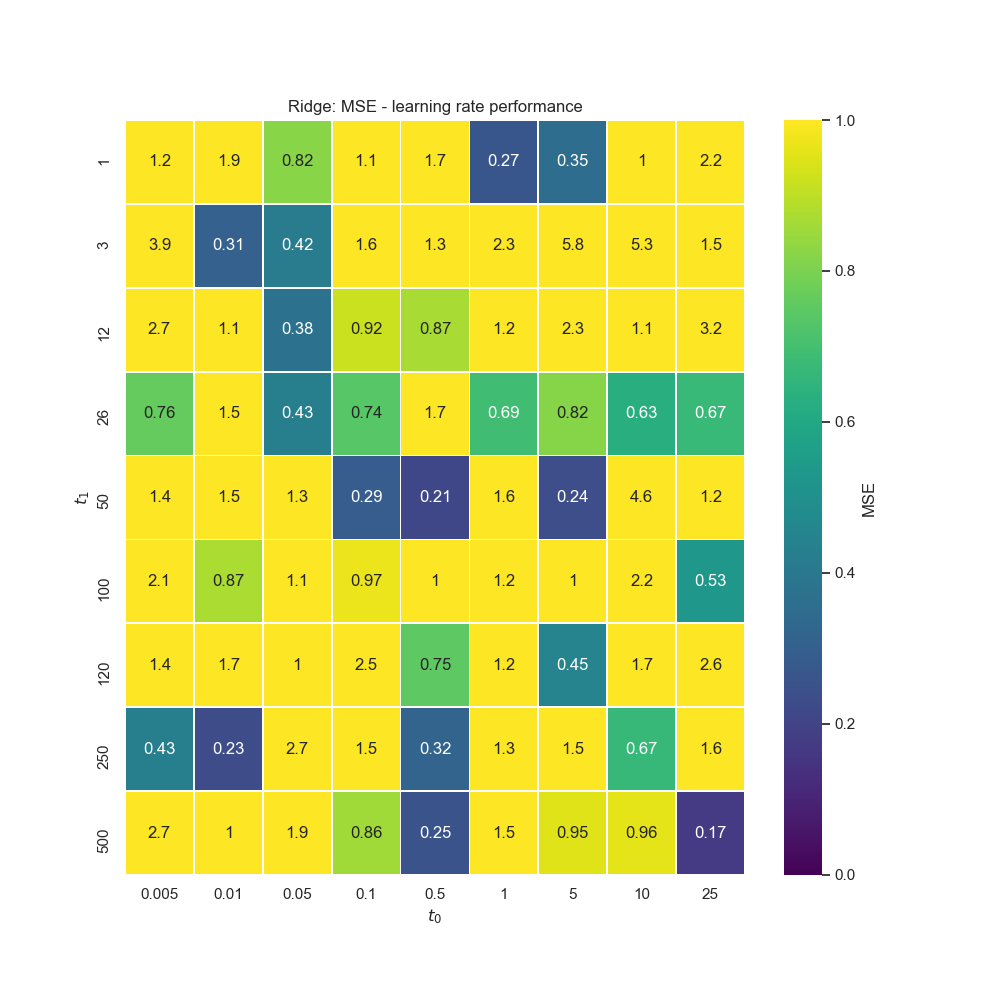
\includegraphics[scale=0.3]{SGD/SGD_eta_Ridge.png}
    \caption{\textbf{Task $a$ – SGD}: MSE performance of the learning rate, choosing a \textit{learning schedule} with parameters $t_0$ and $t_1$. Maximum MSE value set to 1. The optimal values are $t_0 = 25$ and $t_1 = 500$, given an initial learning rate of $\eta_0=5 \ 10^{-2}$.}
    \label{fig:eta0_ridge}
\end{figure}

\begin{figure}[h]
    \centering 
    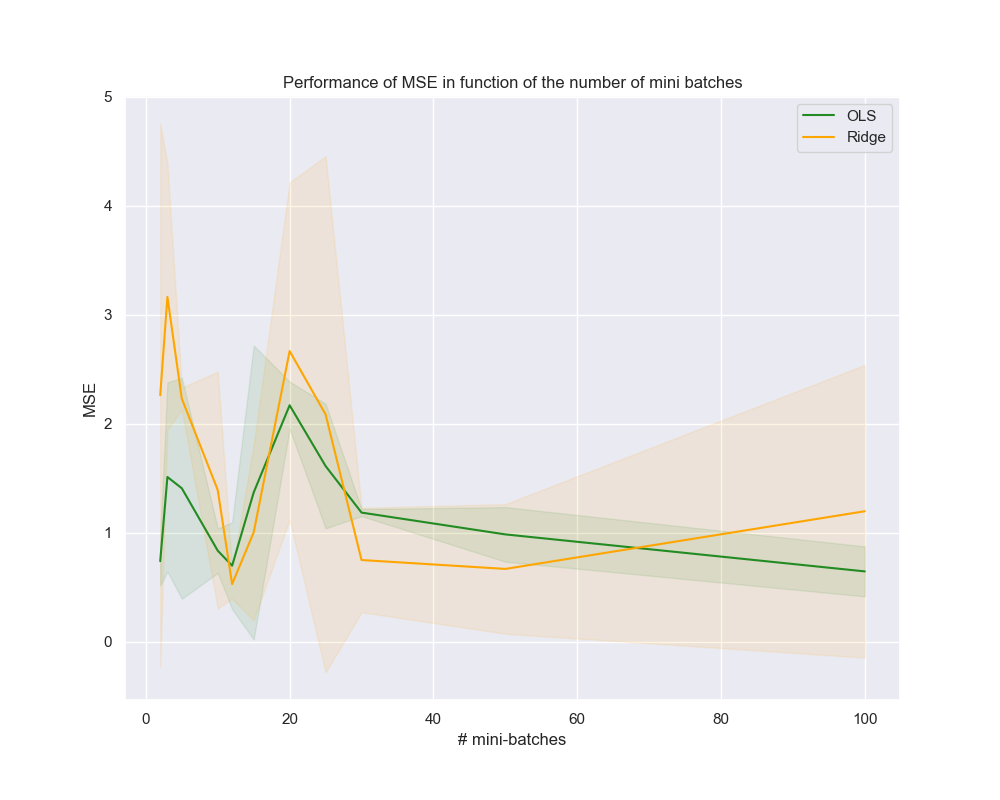
\includegraphics[scale=0.3]{SGD/SGD_minibatches.png}
    \caption{\textbf{Task $a$ – SGD}: MSE performance over the number of minibatches. A rolling mean has been implemented to better appreciate the trend.}
    \label{fig:sgd_mb}

    \centering 
    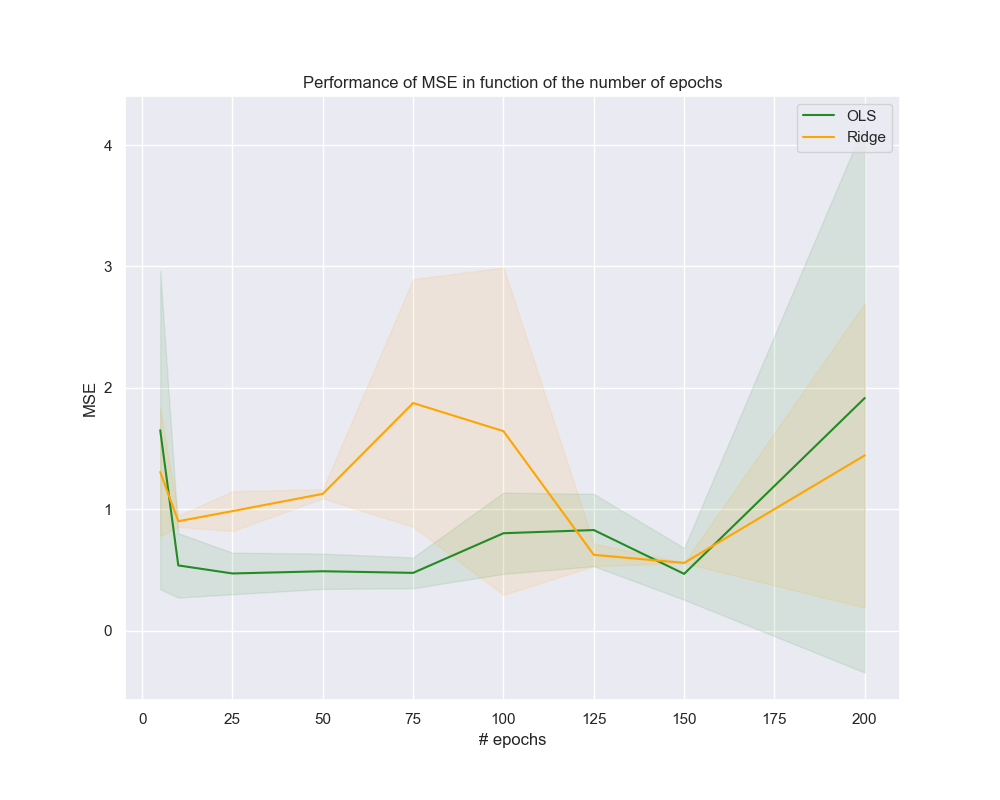
\includegraphics[scale=0.3]{SGD/SGD_epochs.png}
    \caption{\textbf{Task $a$ – SGD}: MSE performance over the number of epochs. A rolling mean has been implemented to better appreciate the trend.}
    \label{fig:sgd_epochs}
\end{figure}

\begin{figure}[h]
    \centering 
    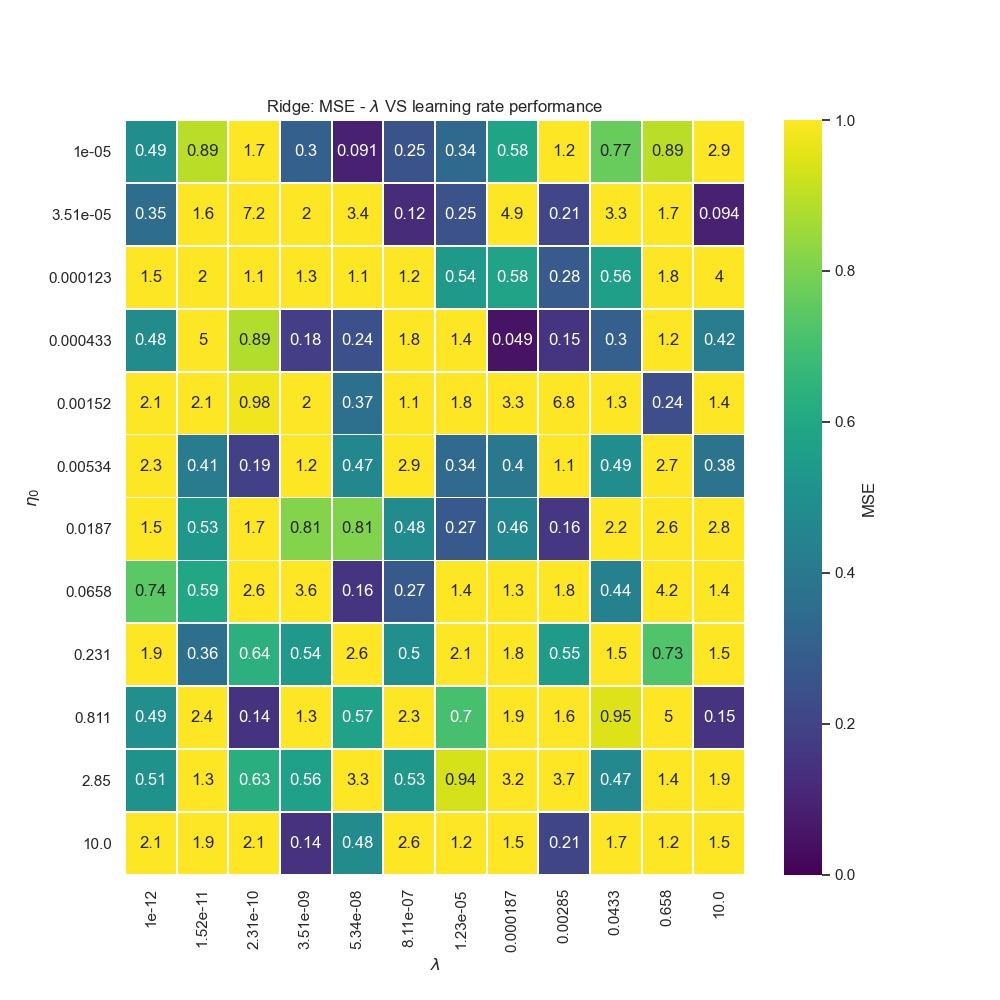
\includegraphics[scale=0.3]{SGD/SGD_lambda_eta.png}
    \caption{\textbf{Task $a$ – SGD}: MSE performance in a cross-investigation over $\lambda$ and the learning rate $\eta$.}
    \label{fig:lmd_eta}
\end{figure}

From the results of this MSE analysis (Figures \ref{fig:eta0_ols}, \ref{fig:eta0_ridge}, \ref{fig:sgd_mb}, \ref{fig:sgd_epochs}) we can then conclude that this implementation of the SGD, choosen a \textit{learning schedule} for the learning rate, shows the best performance for $\eta_0=10^{-5}$ ($t_0, t_1 = 5 \ 10^{-3}, 500$), $n_{minibatches} = 12$, $n_{epochs} = 150$ for OLS, while $\eta_0=5 \ 10^{-2}$ ($t_0, t_1 = 25, 500$), $n_{minibatches} = 50$, $n_{epochs} = 150$ for Ridge. These optimized parameters give a MSE in the order of magnitude minor of $0.1$.

Figures \ref{fig:lmd_eta} shows that the best combination of $\lambda$ and $\eta$ is rispectively $1.87\ 10^{-4}$ and $4.33 \ 10^{-4}$, giving an excellent $MSE=0.049$.

Further comments can be done on the stochastic behaviour in the trends (Figure \ref{fig:sgd_mb}, Figure \ref{fig:sgd_epochs}) (leveled by the rolling mean) when re running the code. A version of the fitting has been implemented with the bootstrap algorithm (\texttt{fitSGD\_BS()}), but the results do not change that much and it's computational more expensive. The reason relies on the intrinsic stochastic character of the SGD algorithm.

\subsection{Neural Network code}

\textit{Write an FFNN code for regression with a flexible number of hidden layers and nodes using the Sigmoid function as activation function for the hidden layers.
Train your network and make an analysis of the regularization parameters and the learning rates employed to find the optimal MSE and R2 scores. Compare the results obtained with the Linear Regression code and your own Neural Network code.}

\textbf{\textit{Note:} The class \texttt{NeuralNetwork} has been implemented for both the Regression and Classification cases but because of a number of unexpected problems I had to face is currently not running yet. The reason relies on the fact that I wished to implement a very versatile class, but I have been trapped myself into the complexity of my own code. Unfortunately this led me to spend several days (weeks) on elaborating this class, lacking on the rest of the project. In order not to be blocked by any progress in the analysis, I'll present here the work I would have done if the code was running. The class credit is to Simone Mirabella, another student of the course, with whom I started structuring the code at the beginning. The class is basically the same as mine, but it runs. The implementation of my class is in the following link: \href{https://github.com/adelezaini/MachineLearning/blob/nn/Projects/Project2/neuralnetwork.py}{https://github.com/adelezaini/MachineLearning/
blob/nn/Projects/Project2/neuralnetwork.py}. Any feedback is more than welcomed! I also apologise for lacking in the depth of the further analysis but the time left was too little to explore more.}

The dataset choosen for this task is the {Boston Housing} because it makes the Neural Network perform on a real case of Regression in Supervised Learning. Firstly the two most correlated features has been selected, the dataset has been splitted into train and test subsets and they have been rescaled by the mean and the standard deviation.

\begin{figure}[h]
    \centering 
    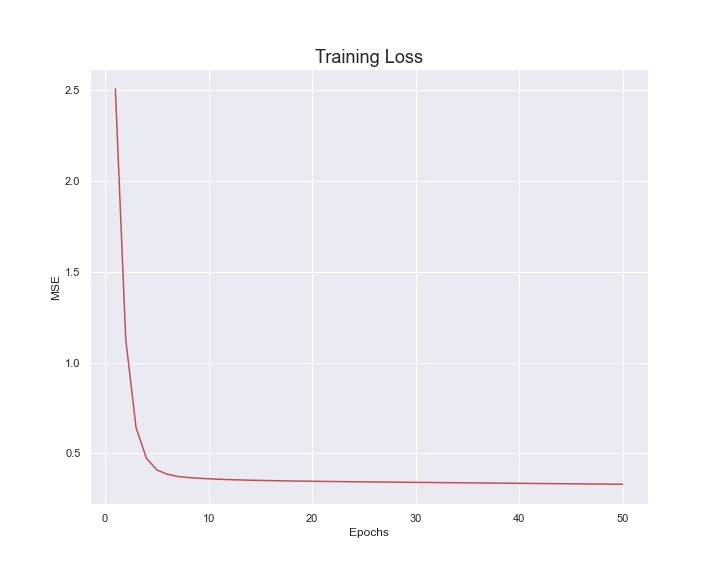
\includegraphics[scale=0.35]{NN/RegrNN_200_50_None_32_50_0.0002.jpg}
    \caption{\textbf{Task $b$ – NN Regression}: Training of the NN with two layers of dimensions $[200,50]$, $n_{epochs}=50$, $n_{minibatches}=32$ and $\eta=0.001$. No regularisation has been considered.}
    \label{fig:train_noreg}
    \centering 
    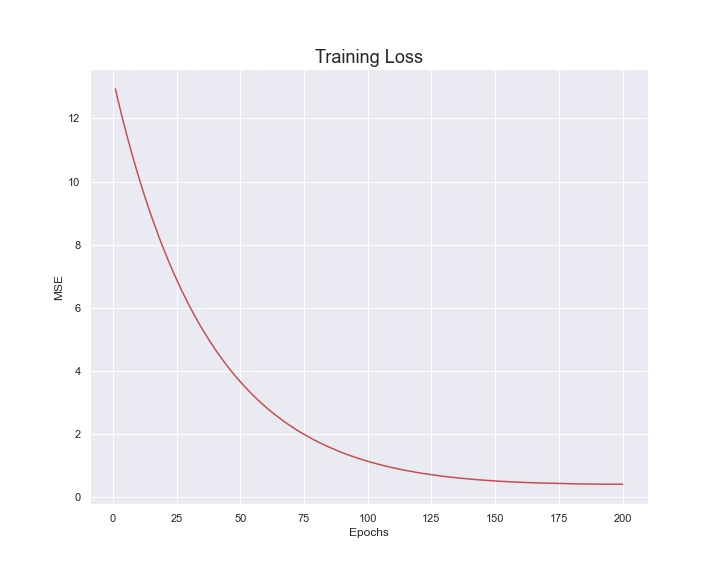
\includegraphics[scale=0.35]{NN/RegrNN_200_50_L2_32_50_0.0002.jpg}
    \caption{\textbf{Task $b$ – NN Regression}: Training of the NN with two layers of dimensions $[200,50]$, $n_{epochs}=200$, $n_{minibatches}=32$ and $\eta=0.01$. 'L2' regularisation has been considered with a $\lambda=0.1$.}
    \label{fig:train_reg}
\end{figure}

\begin{table}[H]
\centering 
\begin{tabular}{@{}ccccc@{}}
& OLS   & Ridge & NN\_no\_reg & NN\_l2\_reg \\ [0.5ex] 
\hline\hline
\multicolumn{1}{|l|}{MSE\_train} & 29.30 & 31.96 & 0.33        & \multicolumn{1}{l|}{0.42} \\ \midrule
\multicolumn{1}{|l|}{MSE\_test}  & 35.35 & 23.05 & 0.61        & \multicolumn{1}{l|}{0.65} \\ \midrule
\multicolumn{1}{|l|}{R2\_test}   & 0.57  & 0.63  & 0.39        & \multicolumn{1}{l|}{0.35} \\ \hline \bottomrule
\end{tabular}
\label{tab:nn_lin}
\caption{\textbf{Task $b$ – NN Regression}: Table summarizing the comparison between Linear and NeuralNetwork methods on the error analysis. The table refers to NN training of Figure \ref{fig:train_noreg} and Figure \ref{fig:train_reg}.}
\label{tab:nn_lin}
\end{table}

\begin{figure}[h]
    \centering 
    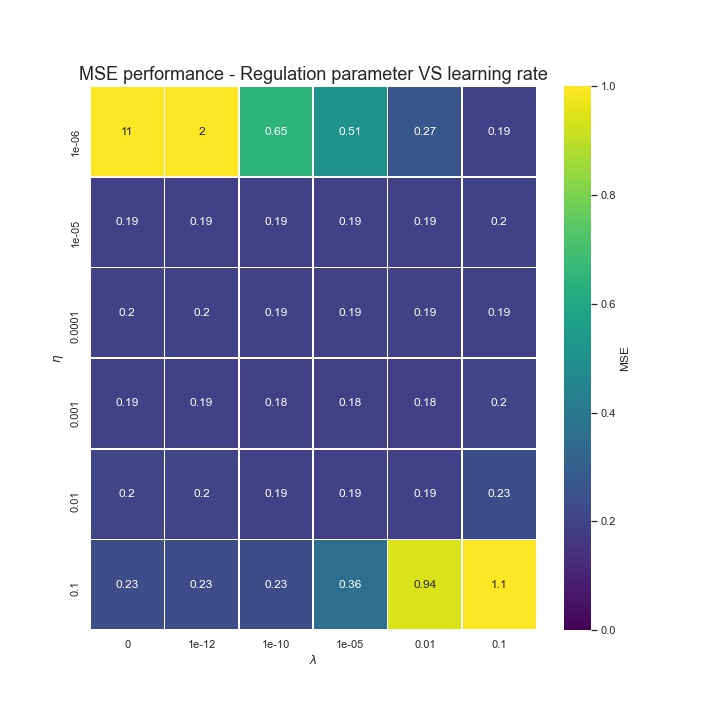
\includegraphics[scale=0.3]{NN/RegrNN_lmd_eta_MSE.jpg}
    \caption{\textbf{Task $b$ – NN Regression}: Cross-investigation on MSE performance of the regularisation parameter $\lambda$ and the learning rate $\eta$.}
    \label{fig:mse_nn_regr}
    \centering 
    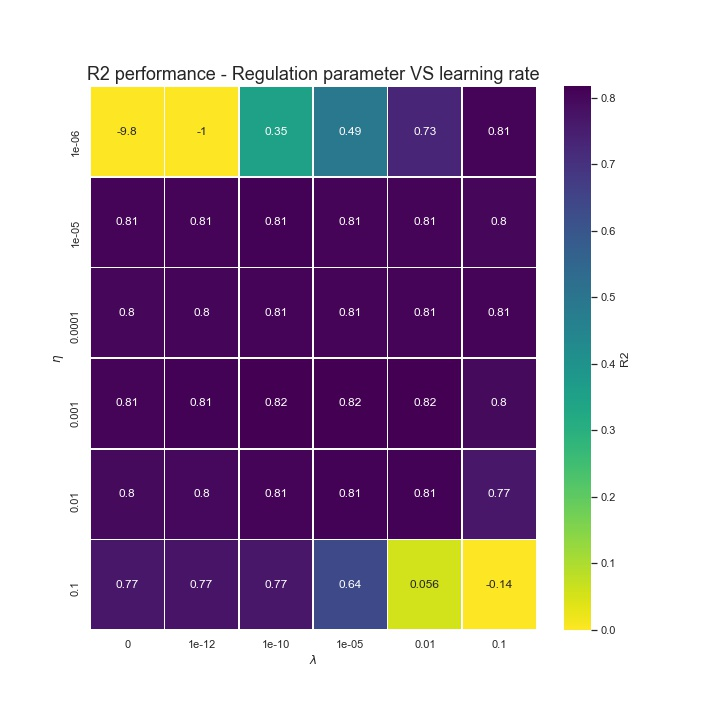
\includegraphics[scale=0.3]{NN/RegrNN_lmd_eta_R2.jpg}
    \caption{\textbf{Task $b$ – NN Regression}: Cross-investigation on R2 performance of the regularisation parameter $\lambda$ and the learning rate $\eta$.}
    \label{fig:r2_nn_regr}
\end{figure}

In the Figures \ref{fig:train_noreg} and \ref{fig:train_reg}, we can appreciate the optimization process of the neural network. On the one hand, the added 'l2' regularisation term can avoid overfitting, on the other hand it leads to a slower convergence of the performance of the network (number of epochs incresed form $50$ to $200$). This is understandable, but the figures have shown an interesting point not deepened before.

The comparison with the Linear Regression (Table \ref{tab:nn_lin}) suggests the excellent performance of the Neural Network, both with or without the regularization option, over the classic Linear Regression methods: the $MSE$ decreases of two orders of magnitude, reaching $0.33$ form $35$. Regarding the optimization of the hyperparameters, we can appreciate from Figures \ref{fig:mse_nn_regr} and \ref{fig:r2_nn_regr} that the neural network best performs with $\eta=0.001$ and $\lambda \in [10^{-12},0.001]$.


\subsection{Testing different activation functions}

\textit{Test different activation functions for the hidden layers. Try out the Sigmoid, the RELU and the Leaky RELU functions and discuss your results. }

\begin{figure}[h]
    \centering 
    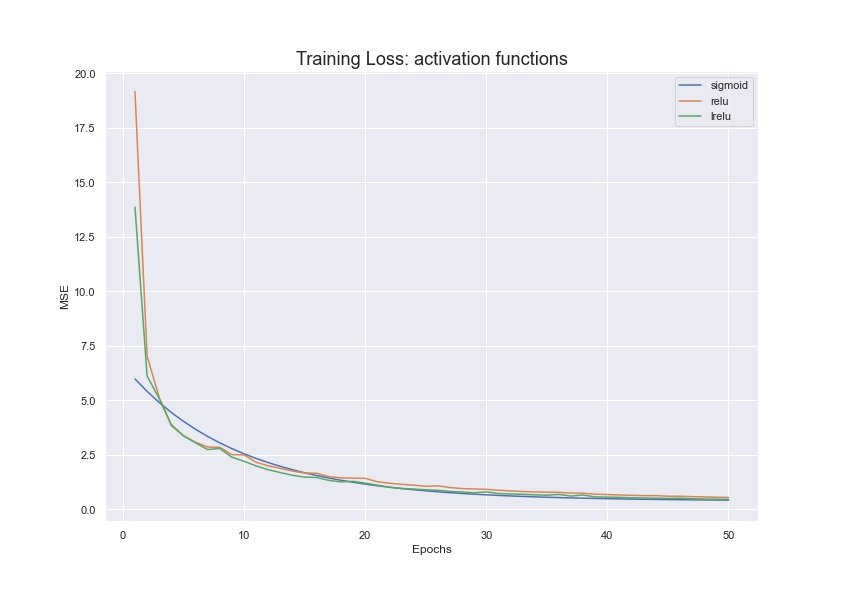
\includegraphics[scale=0.3]{NN/RegrNN_activations.jpg}
    \caption{\textbf{Task $c$ – NN Regression}: Different activation functions of the hidden layers are explored in terms of MSE performance.}
    \label{fig:activations}
\end{figure}

Figure \ref{fig:activations} shows that the choice of the activation function can influence the efficiency at the beginning of the training but that the performance converges to be the same independently by the choosen activation function.

In this particular case no problem is shown, but from literature the choice of the activation function can influence the network's performance.
When the gradients get smaller and smaller as the backpropagation algorithm progresses down to the first hidden layers. As a result, the GD update leaves the lower layer connection weights virtually unchanged, and training never converges to a good solution. This is known in the literature as the vanishing gradients problem. In other cases, the opposite can happen, namely the the gradients can grow bigger and bigger. The result is that many of the layers get large updates of the weights the algorithm diverges. This is the exploding gradients problem. The ranking taken from the literature shows LeakyReLU performing better than ReLU, which performs better than the Sigmoid.

\subsection{Classification  analysis using neural networks}

\textit{Change the code to perform also in the classification casr. Discuss your results and give a critical analysis of the various parameters, including hyper-parameters like the learning rates and the regularization parameter $\lambda$ (as you did in Ridge Regression), various activation functions, number of hidden layers and nodes and activation functions.}

\begin{figure}[h]
    \centering 
    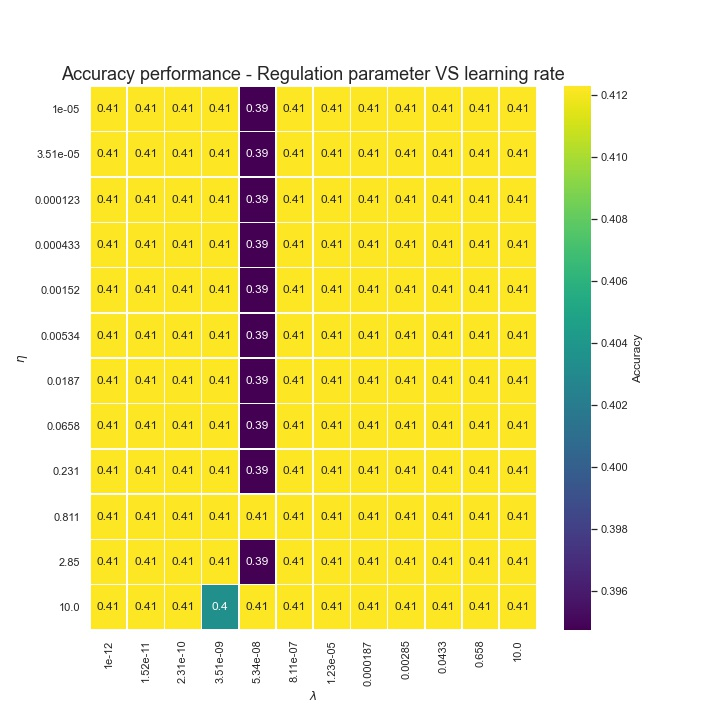
\includegraphics[scale=0.3]{Class/ClassNN_lmd_eta.jpg}
    \caption{\textbf{Task $d$ – NN Classification}: Grid-search on Accurancy performance of the regularisation parameter $\lambda$ and the learning rate $\eta$.}
    \label{fig:acc_lmd_eta}
\end{figure}

\begin{figure}[h]
    \centering 
    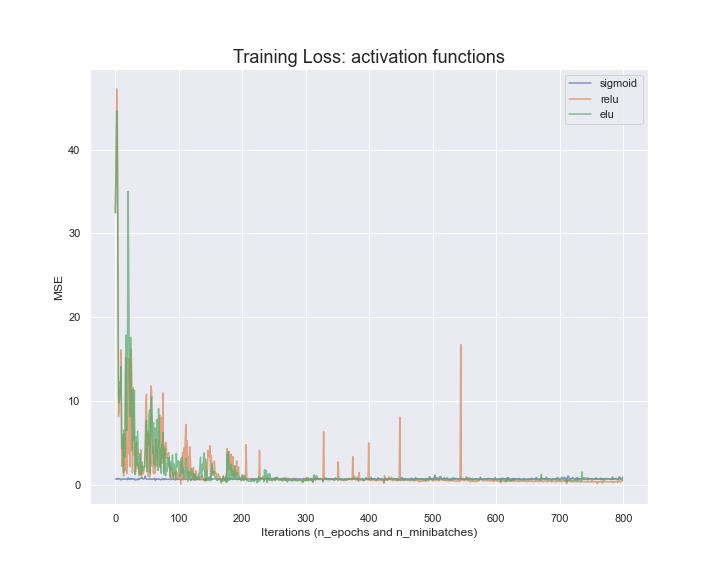
\includegraphics[scale=0.3]{Class/ClassNN_activations.jpg}
    \caption{\textbf{Task $d$ – NN Classification}: Different activation functions of the hidden layers are explored in terms of training performance performance. At the end the Sigmoid and eLU function has an accurancy of $0.412$, while ReLU of $0.096$.}
    \label{fig:activations_class}
\end{figure}

While training the network, the user can learn how to better set the number of hidden layers and number of neurons in each layer. Increasing the number of hidden layers does not increase the performance consistently, while the pattern of the number of neurons throughout the hidden layers seems more important. Starting from a number close to the input dimension and go progressively to the number of the outputs gives the best results in terms of performance.

%\subsection{Logistic Regression code}

%\textit{Compare the FFNN code with Logistic regression.}

%The class has been implemented but the comparison with the Neural Network is left for a future development.


% ===========================================
\section{Conclusion}\label{sec:conclusion}

\textit{This last section covers task f of the project: Critical evaluation of the various algorithms.}

In this report we explored the performance of the neural networks and related algorithms, compared to standard techniques. We can state that overall the neural network can lead to excellent results, when optimizing properly the parameters and the network architecture. 

Most of the work behind this report has been focused on the implementation of the project, compared to the analysis and optimization of the parameters for which little time was left. Yet some interesting results can be highlighted. Starting from the SGD algorithm, the analysis shows the best performance when considering optimal values for the different parameters: $\eta_0=10^{-5}$, $n_{minibatches} = 12$, $n_{epochs} = 150$ for the OLS Regression, while $\eta_0=5 \ 10^{-2}$, $n_{minibatches} = 50$, $n_{epochs} = 150$ for the Ridge Regression. Figures \ref{fig:lmd_eta} shows that the best combination for the Ridge of $\lambda$ and $\eta$ is respectively $1.87\ 10^{-4}$ and $4.33 \ 10^{-4}$, giving an excellent $MSE=0.049$. All the figures manifest the intrisic stochastic behaviour of the algorithm.

Regarding the neural network, we can appreciate its better performance over the classical method of Linear Regression (Table \ref{tab:nn_lin}), in particular considering as hyperparameters $\eta=0.001$ and $\lambda \in [10^{-12},0.001]$ (Figures \ref{fig:mse_nn_regr} and \ref{fig:r2_nn_regr}). The choice of the activation function does not seem to influence consistently the performance when training the network over several iterations (Figures \ref{fig:activations} and \ref{fig:activations_class}). As regarding the Classification case, little has been explored but it shows a good flexibility on the choice of the hyperparameters and activation function, but overall the accurancy never exceeds $0.42$. This is an interesting point to explore.

Surely we can consider this work still open to improvements. Starting from fixing the code and filling the gaps, but also on the analysis of the performance. It would be very interesting to better explore the optimization and regularization algorithms, several combinations of number of hidden layers and respective neurons, various kinds of learning rate and choices of the input datasets, but also implementing new methods, such as the Batch Normalization, the Dropout or the Gradient Clipping.

\newpage
\newpage
% ===========================================
\section*{References}\label{sec:references}
\begin{itemize}
    \item[-] \href{https://compphysics.github.io/MachineLearning/doc/web/course.html}{FYS-STK3155 courses' notes}
    \item[-] \href{https://static.latexstudio.net/article/2018/0912/neuralnetworksanddeeplearning.pdf}{Michael Nielsen, Neural Networks and Deep Learning}
    \item[-] \href{https://github.com/UdiBhaskar/Deep-Learning}{UdiBhaskar/Deep-Learning GitHub repository}
    \item[-] \href{https://datascience-enthusiast.com/DL/Logistic-Regression-with-a-Neural-Network-mindset.html}{Fisseha Berhane, Logistic Regression with a Neural Network mindset}
    \item[-] \href{https://ml-cheatsheet.readthedocs.io/en/latest/index.html}{ML Glossary}
    \item[-] \href{https://www.youtube.com/watch?v=Ilg3gGewQ5U}{3Blue1Brown, What is backpropagation really doing? | Chapter 3, Deep learning}
    \item[-] \href{https://ruder.io/optimizing-gradient-descent/index.html#stochasticgradientdescent}{Sebastian Ruder, An overview of gradient descent optimization algorithms}
    \item[-] \href{https://towardsdatascience.com/stochastic-gradient-descent-clearly-explained-53d239905d31}{Medium, Aishwarya V Srinivasan, Stochastic Gradient Descent — Clearly Explained}
    \item[-] \href{https://medium.com/@zeeshanmulla/cost-activation-loss-function-neural-network-deep-learning-what-are-these-91167825a4de}{Medium, Mohammed Zeeshan Mulla, Cost, Activation, Loss Function|| Neural Network|| Deep Learning. } 
    \item[-] \href{http://neuralnetworksanddeeplearning.com/chap2.html}{Michael Nielsen, How the backpropagation algorithm works} 
    \item[-] \href{https://neptune.ai/blog/cross-entropy-loss-and-its-applications-in-deep-learning}{Author Rose Wambui,Cross-Entropy Loss and Its Applications in Deep Learning.} 
    \item[-] \href{https://sophiamyang.github.io/DS/optimization/multiclass-logistic/multiclass-logistic.html}{Sophia Yang, Multiclass logistic regression from scratch.} 
    \item[-] \href{https://jovian.ai/attyuttam/03-logistic-regression}{Image Classification using Logistic Regression in PyTorch} 

\end{itemize}
%%https://blogs.egu.eu/divisions/cr/2017/01/25/katabatic-winds-a-load-of-hot-or-cold-air/
%https://slideplayer.com/slide/16538958/
%https://www.weather.gov/media/zhu/ZHU_Training_Page/clouds/stability_clouds/stability_clouds.pdf
%http://www.arpalazio.net/main/aria/didattica/corso01/Capitolo_02_2010.pdf

\begin{thesitography}
\item \textit{Courses notes}: <\url{https://compphysics.github.io/MachineLearning/doc/web/course.html}>

\bibitem{image2}  Thomson Higher Education, 2007; \\ URL: \url{https://www.weather.gov/media/zhu/ZHU_Training_Page/clouds/} \\ \url{stability_clouds/stability_clouds.pdf} \\ Data ultimo accesso: 9 febbraio 2020.

\bibitem{image3}  \textit{Modello fluidodinamico del PBL}, ARPA Lazio; \\ URL: \url{http://www.arpalazio.net/main/aria/didattica/corso01/Capitolo_} \\ \url{02_2010.pdf} \\ Data ultimo accesso: 9 febbraio 2020.

\bibitem{image4}  \textit{Katabatic winds–A load of hot (or cold) air?}, Cryospheric Science, EGU Blogs; \\ URL: \url{https://blogs.egu.eu/divisions/cr/2017/01/25/katabatic-winds-} \\ \url{a-load-of-hot  -or-cold-air}\\ Data ultimo accesso: 9 febbraio 2020.

\bibitem{image5}  \textit{Lo splendore dei ghiacci – La suggestione e l'inquietudine dei ghiacci perenni}, \\ Massimo Dei Cas, Paesi di Valtellina e Valchiavenna; \\ URL: \url{http://www.paesidivaltellina.it/ghiacci/index.htm}\\ Data ultimo accesso: 12 febbraio 2020.

\bibitem{image6} Comitato Glaciologico Italiano – GLIMS project; \\ URL: \url{http://repo.igg.cnr.it/ghiacciaiCGI/ghiacciai_new.html}\\ Data ultimo accesso: 12 febbraio 2020.

\end{thesitography}


% ===========================================

\clearpage

\onecolumngrid

\bibliographystyle{apalike}
\bibliography{Bibliography.bib}


\end{document}

